\documentclass{beamer}


\usepackage{amsmath}
\usepackage{physics}
\usepackage{color}
\usepackage{graphicx}
\usepackage{hyperref}

%\usetheme{Copenhagen}
%\usetheme{Warsaw}
\usecolortheme{crane}
\beamertemplatenavigationsymbolsempty

\setbeamertemplate{itemize items}[circle]
\setbeamertemplate{enumerate items}[circle]

\title{Quantum Research Project}
\author{Pierriccardo Olivieri}
\institute{Politecnico di Milano}

\titlegraphic{
    
\includegraphics[scale=0.2]{img/logo.png}
    \centering}

\begin{document}

\maketitle


\begin{frame}
    \frametitle{outline}
    \begin{itemize}
        \item Random/Quantum walk intro
        \item Coined DTQW in cycle graph 
        \item Results
        \item Generalization
        \item Performance
        \item Szegedy Quantum Walks
        \item Applications 
        \item Conclusions
    \end{itemize}
\end{frame}

\begin{frame}
    \frametitle{What is a Random walk?}
    \begin{definition}[Random walk]
        Is a mathematical object that describe a random path over a mathematical space 
    \end{definition}
    We can identify two type of Random Walk
    \begin{itemize}
        \item discrete time 
        \item continous time 
    \end{itemize}
    
\end{frame}

\begin{frame}
    \frametitle{Random Walk on a line}
    \begin{example}[Random walk on a line]
        \begin{itemize}
            \item line of integer numbers $\mathbb{Z}$
            \item walker position
            \item random experiment
            \item move the walker
        \end{itemize}
    \end{example}

    \begin{figure}[h!]
        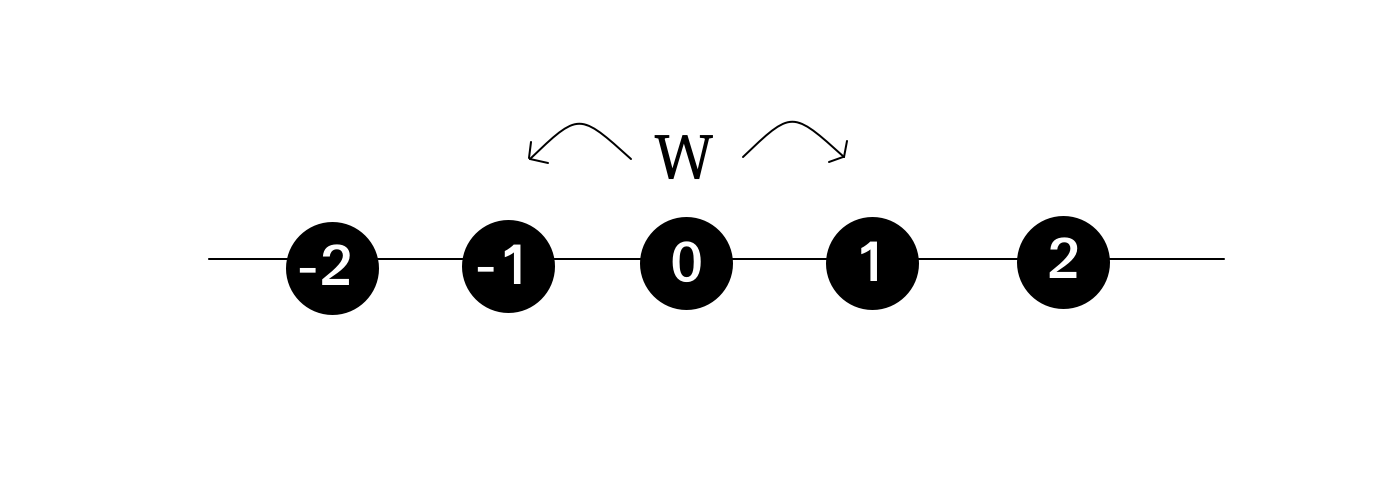
\includegraphics[scale=0.3]{img/random_walk_line.png}
        \centering
    \end{figure}
\end{frame}

\begin{frame}
    \frametitle{Quantum Walks}
    Analogous of random walks, again the focus is on Discrete time quantum walks

    \begin{example}[quantum walk on a line]
        To construct a Quantum walk on a line we need
        \begin{itemize}
            \item mathematical space
            \item position
            \item coin operator
            \item shift operator
            \item state of the system
        \end{itemize}
    \end{example}

    \begin{figure}[h!]
        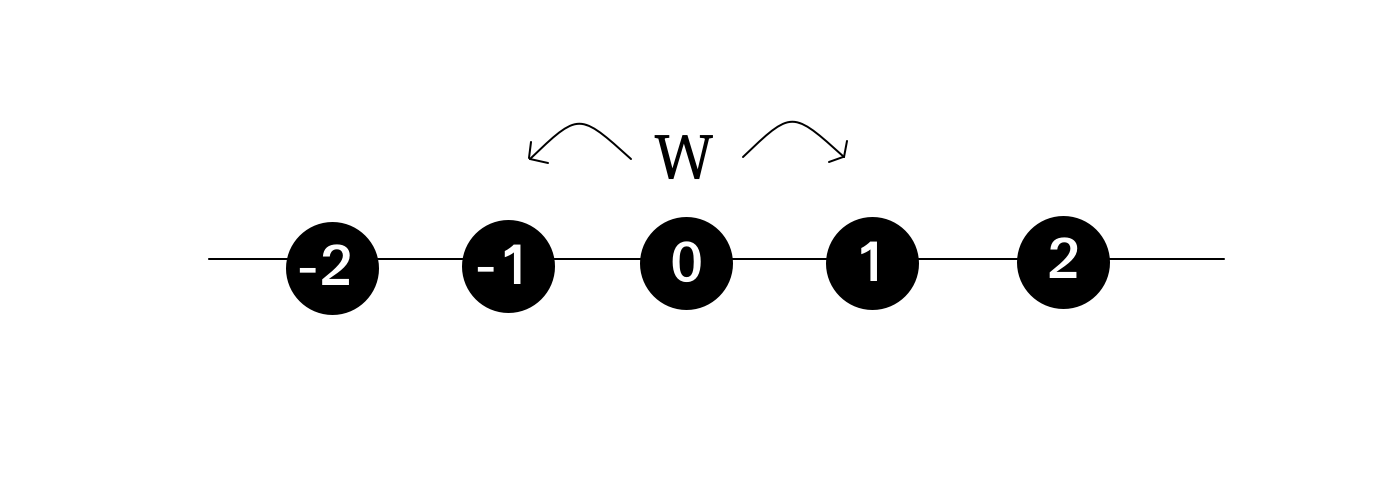
\includegraphics[scale=0.2]{img/random_walk_line.png}
        \centering
    \end{figure}
    there are also model without coin
\end{frame}


\begin{frame}
    \frametitle{Mathematical space}
    The space in which the Coined QW is defined is defined by the Hilbert space
    \begin{equation}
        \mathcal{H}=\mathcal{H}_{p}\otimes\mathcal{H}_{c}
    \end{equation}
    where $\mathcal{H}_{p}$ and $\mathcal{H}_{p}$ are the Hilbert spaces 
    of the coin and position  
\end{frame}

\begin{frame}
    \frametitle{Position}
    \textbf{Position} identified by vector:
    \begin{equation}
        \ket{position} \in \mathcal{H}_{p}
    \end{equation} 
    encoding in binary labels we need Log(N) qubits to reresent the number.

    \begin{example}[$N < 8 => 3 qubits$]
        \begin{itemize}
            \item $0 -> 000 -> \ket{000}$
            \item $1 -> 100 -> \ket{100}$
            \item $7 -> 111 -> \ket{111}$
        \end{itemize}
    \end{example}    
\end{frame}

\begin{frame}
    \frametitle{Coin operator \& state of the system}
    The \textbf{coin operator} is a vector in a 2-dimensional Hilbert space 
    \begin{equation}
        \ket{coin} \in \mathcal{H}_{c} \,\,\,\, where \mathcal{H}_{c} = \ket{0}, \ket{1}
    \end{equation}
    
    Combining element defined before a \textbf{state} of the system is:
    \begin{equation}
        \ket{\phi_{initial}} = \ket{position}_{initial} \otimes \ket{coin}_{initial}
    \end{equation}
\end{frame}

\begin{frame}
    \frametitle{Shift operator}
    The operator that actually perform the shift of the walker depending on the outcome of the coin
    \begin{equation}
        \scriptstyle S = \ket{0}_{c} \bra{0} \otimes \sum{i} \ket{i + 1}_{p} \bra{i} + \ket{1}_{c} \bra{1} \otimes \sum{i} \ket{i - 1}_{p} \bra{i} 
    \end{equation}
\end{frame}

\begin{frame}
    \frametitle{Coined quantum walk operator}
    Combining the element defined before we obtain the operator that perform one step of the 
    quantum walk:
    \begin{equation}
        U = S x (C \otimes I_{p}) = SC
    \end{equation}
\end{frame}

\begin{frame}
    \frametitle{Coined DTQW on a cycle graph}
    Now we want to implement the Coined DTQW on a cycle graph with N = 8

    \begin{columns}[T]
        \begin{column}{.5\textwidth}
            \begin{block}{Circuit:}
                \begin{itemize}
                    \item position encoded in 3 qubits e.g. $7 -> \ket{111}$
                    \item coin operator: Hadamard coin (1 qubit)
                    \item shift operator $\ket{i + 1}$ or $\ket{i - 1}$
                \end{itemize}
            \end{block}
        \end{column}
        \begin{column}{.5\textwidth}
            \begin{block}{Cycle Graph $C_{8}$}
                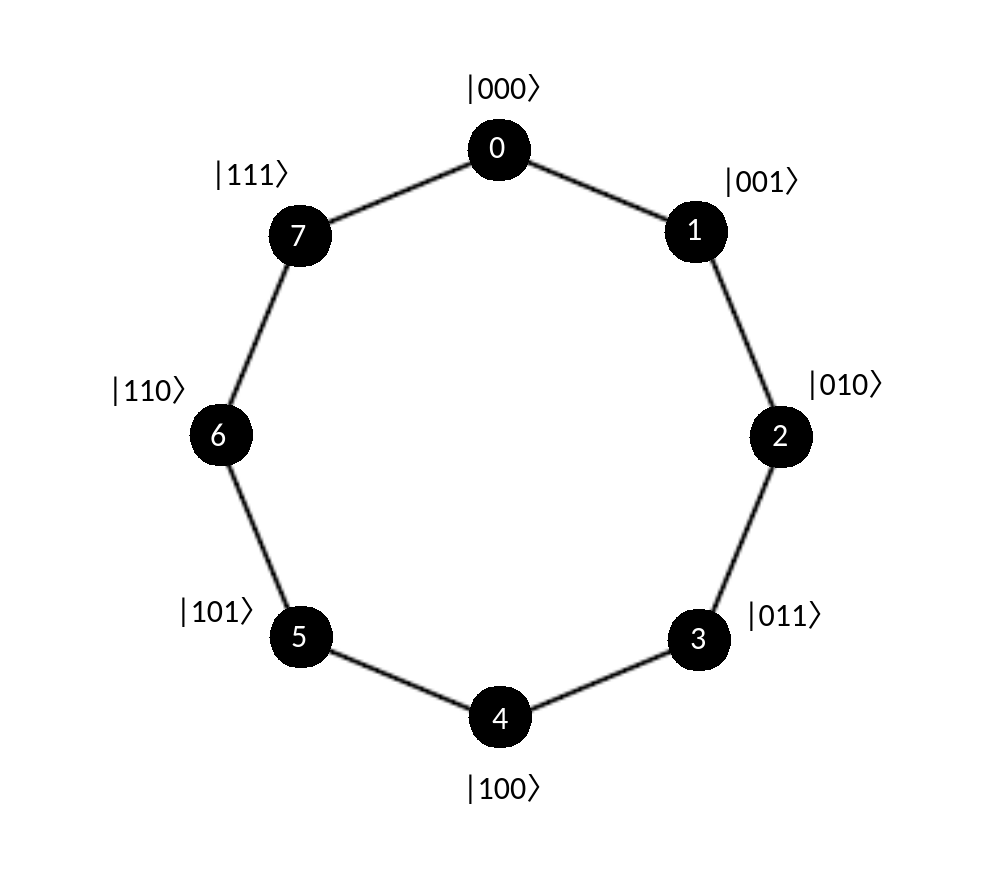
\includegraphics[scale=0.2]{img/cyclic_graph.png}
                \centering
            \end{block}
        \end{column}
    \end{columns}
\end{frame}

\begin{frame}
    \frametitle{Circuit implementation}
    We need 3 element to construct the circuit:
    \begin{columns}[T]
        \begin{column}{.5\textwidth}
            \begin{block}{Circuit Components}
                \begin{itemize}
                    \item increment circuit
                    \item decrement circuit
                    \item Hadamard gate
                \end{itemize}
            \end{block}
        \end{column}
        \begin{column}{.5\textwidth}
            \begin{block}{Final Circuit}
                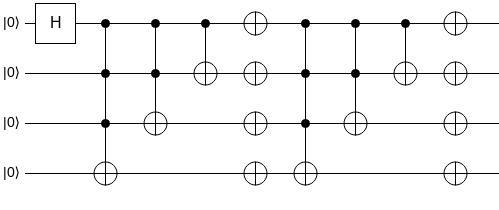
\includegraphics[scale=0.4]{img/cqw.jpg}
            \end{block}
        \end{column}
    \end{columns}   

\end{frame}

\begin{frame}
    \frametitle{Increment circuit}
    \begin{figure}[h!]
        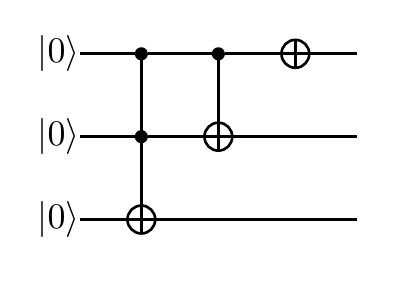
\includegraphics[scale=0.7]{img/increment_circuit.png}
        \centering
    \end{figure}
\end{frame}

\begin{frame}
    \frametitle{Decrement circuit}
    \begin{figure}[h!]
        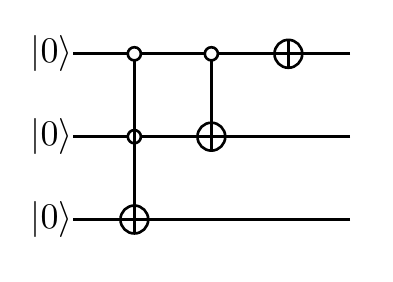
\includegraphics[scale=0.5]{img/decrement_circuit.png}
        \centering
    \end{figure}
    \begin{figure}[h!]
        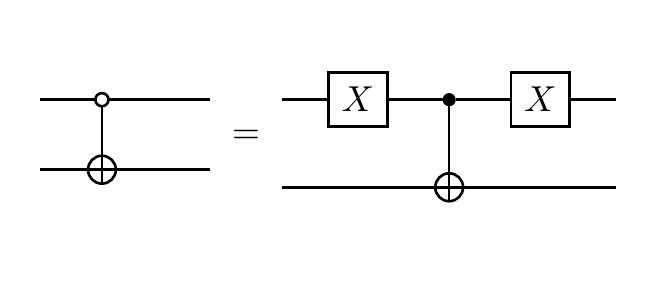
\includegraphics[scale=0.3]{img/ncn_equiv.png}
        \centering
    \end{figure}
\end{frame}

\begin{frame}
    \frametitle{Decrement circuit}
    \begin{figure}[h!]
        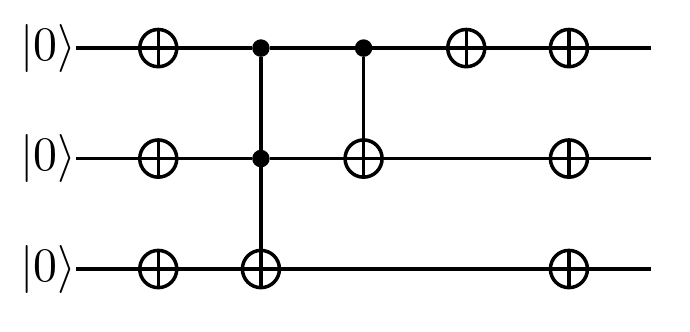
\includegraphics[scale=0.5]{img/decr.png}
        \centering
    \end{figure}
\end{frame}

\begin{frame}
    \frametitle{Complete circuit}
    \begin{figure}[h!]
        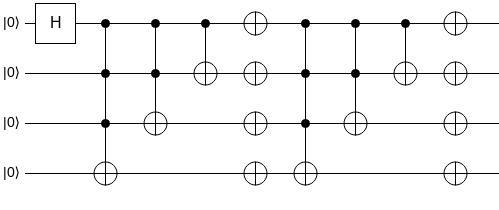
\includegraphics[scale=0.5]{img/cqw.jpg}
        \centering
    \end{figure}
    \begin{figure}[h!]
        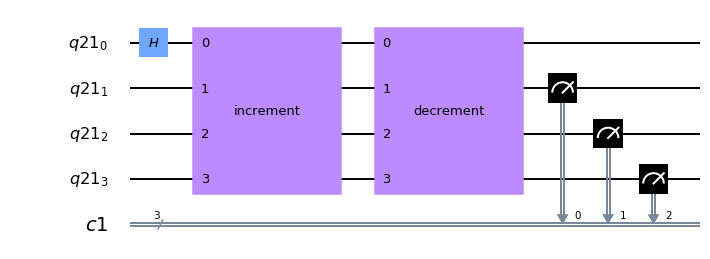
\includegraphics[scale=0.4]{img/cqwqiskit.png}
        \centering
    \end{figure}
    
    \href{https://bit.ly/36uuySe}{Click here for Quirk Simulation}
\end{frame}

\begin{frame}
    \frametitle{Results}
    To perform a Quantum walk we apply the circuit several times starting 
    from a certain position

    \begin{columns}[T]
        \begin{column}{.4\textwidth}
            \begin{block}{Results}
                \begin{itemize}
                    \item true randomness behavior (vs classic gaussian)
                    \item probability of measure odd number starting from an even is close to zero
                    \item Hadamard coin treats two direction in different way
                \end{itemize}
            \end{block}
        \end{column}
        \begin{column}{.6\textwidth}
            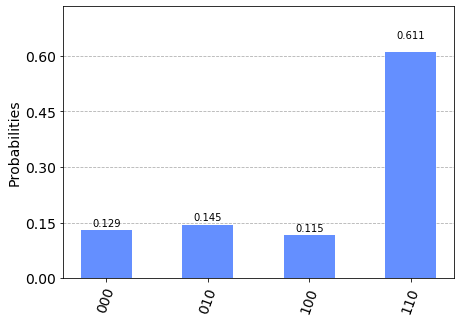
\includegraphics[scale=0.3]{img/100_steps_walk.png}
            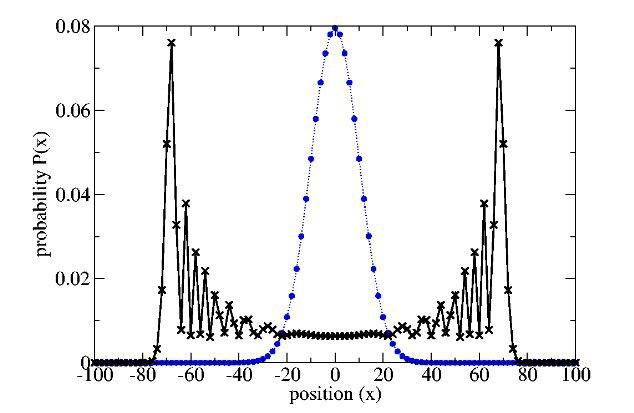
\includegraphics[scale=0.3]{img/dist.jpg}
        \centering
        \end{column}
    \end{columns}
\end{frame}

\begin{frame}
    \frametitle{Generalization}
    Two Generalization anlysis
    \begin{columns}[T]
        \begin{column}{.5\textwidth}
            \begin{block}{w.r.t. model}
                \begin{itemize}
                    \item different type of coin (or model without coin)
                    \item different type of shift operator
                    \item Generalization for dimensions > 1
                \end{itemize}
            \end{block}
        \end{column}
        \begin{column}{.5\textwidth}
            \begin{block}{w.r.t. to class graph}
                \begin{itemize}
                    \item increasing nodes number we need ancillary qubits
                    \item each graph/graph class needs a specific circuit 
                \end{itemize}
            \end{block}
        \end{column}
    \end{columns}
    
\end{frame}

\begin{frame}
    \frametitle{Multi controlled gates}
    \begin{columns}
        \begin{column}{.5\textwidth}
            \begin{itemize}
                \item \small are difficult to implement
                \item \small implementation may require ancillary qubits
                \item \small various type (ancillary, rotations)
                \item \small can lead to inefficiency of the circut
            \end{itemize}
        \end{column}
        \begin{column}{.5\textwidth}
            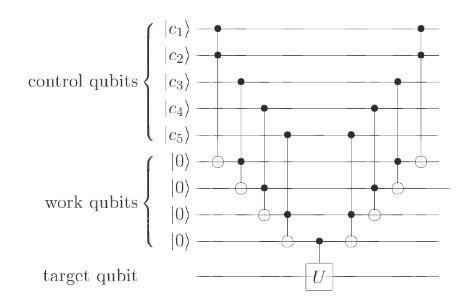
\includegraphics[scale=0.4]{img/ancillary.jpg}
        \centering
        \end{column}
    \end{columns}

    \begin{figure}[h!]
        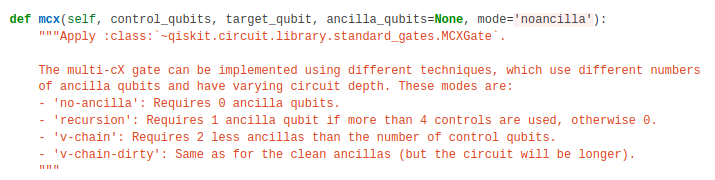
\includegraphics[scale=0.5]{img/mcx.png}
        \centering
    \end{figure}
\end{frame}



\begin{frame}
    \frametitle{Performance}
    \begin{definition}[Search problem]
        find a marked vertex in a graph using Quantum Walks
        and measure where the probability of find it is high
    \end{definition}
    Concepts to consider to comapre performance w.r.t. classic
    \begin{itemize}
        \item \small Comparison made by consider total number of queries to a fixed oracle
        \item \small Efficiency of the circuit at most O(Poly(log(N))) two and one qubit gates
        \item \small Considered efficient if a quadratic speedup is possble wrt classical best search
        \item \small A speedup is possble w.r.t. some class of graphs (hypercube, toroid...)
    \end{itemize}

\end{frame}

\begin{frame}
    \frametitle{Limitations}
    This method is limited to certain type of graphs:
    \begin{itemize}
        \item undirected graph
        \item wighted graphs
    \end{itemize}
    To overcome this limitations we need another model: Szegedy QW
\end{frame}


\begin{frame}
    \frametitle{Markow Chain}
    A Markow chain is
    \begin{itemize}
        \item Stochastic process
        \item sequence of random variables
        \item $P(X_{n} | X_{n-1}, X_{n-2},...,X_{n-N}) = P(X_{n} | X_{n-1})$
        \item if time-independent can be represented by a Transition Matrix P
        \item we can represent our graph with this 
    \end{itemize} 

\end{frame}

\begin{frame}
    \frametitle{Graph representation}
    We can represent our graph with the Adjacency matrix
    \begin{equation}
        A_{i,j} = 
        \begin{cases} 
            1\, if (v_{i}, v_{j}) \in E \\
            0\, otherwise
        \end{cases}
    \end{equation}
    \begin{equation*}
        A =
        \begin{pmatrix}
        0 & 1 & 0 & 0 & 0 & 0 & 0 & 1 \\
        0 & 0 & 1 & 0 & 0 & 0 & 1 & 0 \\
        0 & 1 & 0 & 1 & 0 & 0 & 0 & 0 \\
        0 & 0 & 1 & 0 & 1 & 0 & 0 & 0 \\
        0 & 0 & 0 & 1 & 0 & 1 & 0 & 0 \\
        0 & 0 & 0 & 0 & 1 & 0 & 1 & 0 \\
        0 & 0 & 0 & 0 & 0 & 1 & 0 & 1 \\
        1 & 0 & 0 & 0 & 0 & 0 & 1 & 0 \\
        \end{pmatrix}
    \end{equation*}
\end{frame}

\begin{frame}
    \frametitle{Graph representation}
    Then we can construct the Transition matrix using as probability
    this equation:
    \begin{equation}
        P_{i,j} = \frac{A_{i,j}}{indeg(j)}
    \end{equation}
    And we obtain:    
    \begin{equation*}
        P = \frac{1}{2}
        \begin{pmatrix}
        0 & 1 & 0 & 0 & 0 & 0 & 0 & 1 \\
        0 & 0 & 1 & 0 & 0 & 0 & 1 & 0 \\
        0 & 1 & 0 & 1 & 0 & 0 & 0 & 0 \\
        0 & 0 & 1 & 0 & 1 & 0 & 0 & 0 \\
        0 & 0 & 0 & 1 & 0 & 1 & 0 & 0 \\
        0 & 0 & 0 & 0 & 1 & 0 & 1 & 0 \\
        0 & 0 & 0 & 0 & 0 & 1 & 0 & 1 \\
        1 & 0 & 0 & 0 & 0 & 0 & 1 & 0 \\
        \end{pmatrix}
    \end{equation*}
\end{frame}

\begin{frame}
    \frametitle{Szegedy Quantum Walk}
    \begin{columns}
        \begin{column}{.5\textwidth}
            We need to define the components like in the Coined case:
            \begin{block}{Components}
                
                \begin{itemize}
                    \item mathematical space
                    \item state vector
                    \item swap operator
                    \item Reflection operator
                \end{itemize}
            \end{block}
        \end{column}
        \begin{column}{.5\textwidth}
            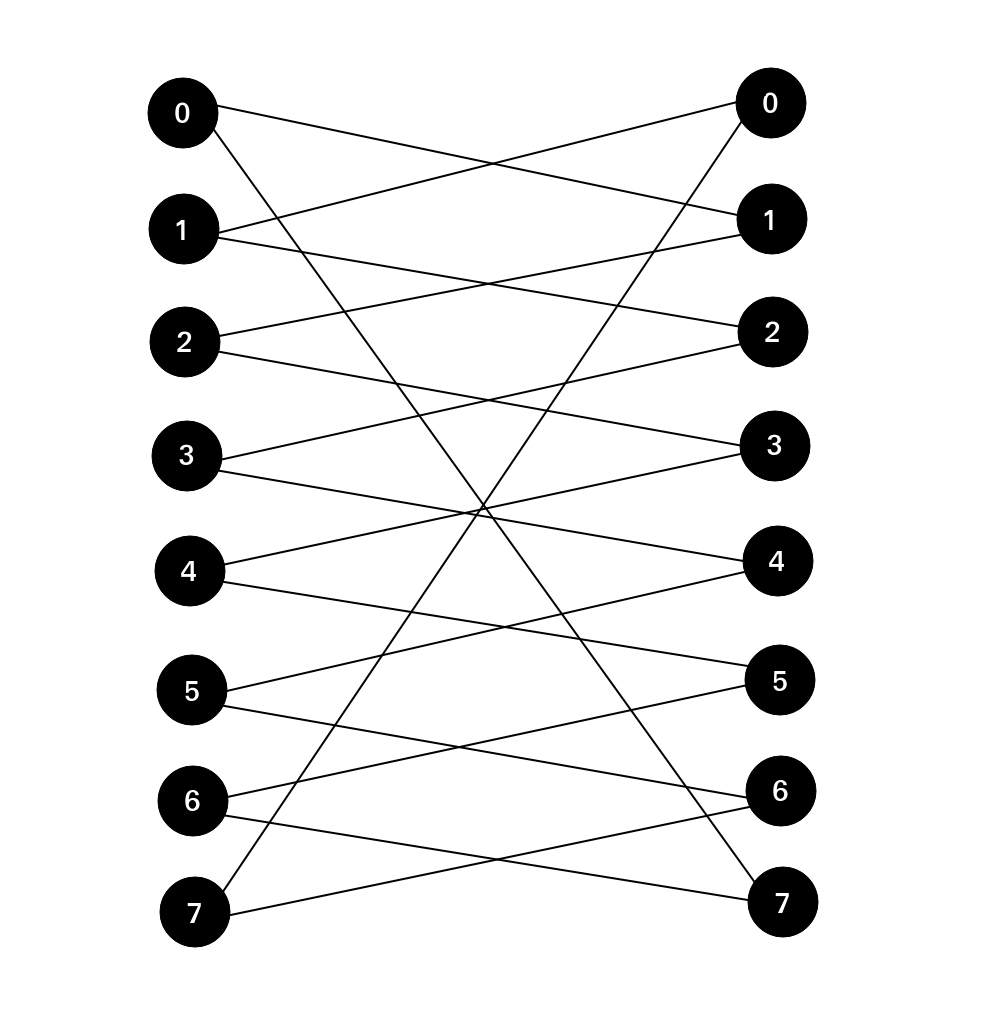
\includegraphics[scale=0.25]{img/bipartite.png}
            
        \end{column}
    \end{columns}
\end{frame}

\begin{frame}
    \frametitle{Szegedy Quantum Operator}
    
    The \textbf{mathematical space} for this operator is:
    \begin{equation}
        \mathcal{H} = \mathcal{H}_{2}^{N} \otimes \mathcal{H}_{2}^{2}
    \end{equation}
    Where N is the number of nodes, thus $\mathcal{H}$ has dimension $N^{2}$ 
    Here the state vector is compoed of two vector $R_{1}$ and $R_{2}$

\end{frame}

\begin{frame}
    \frametitle{State vector \& Swap Operator}
    The \textbf{state vector} that represent the system is:
    \begin{equation}
        \ket{\psi} = \sum_{i=0}^{N-1}\sum_{j=0}^{N-1} a_{i,j}\ket{i,j} 
    \end{equation}
    
    The \textbf{Swap operator} S given by:
    
    \begin{equation}
        \mathcal{S} = \sum_{i=0}^{N-1}\sum_{j=0}^{N-1} \ket{i,j}\bra{j,i} 
    \end{equation}
    
\end{frame}

\begin{frame}
    \frametitle{Reflection Operator}
    Then we define the projector states of the markow chain:
    
    \begin{equation}
        \ket{\psi_{i}} = \ket{i} \otimes \sum_{j=0}^{N-1}\sqrt{P_{j+1,i+1}}\ket{j} \equiv \ket{i} \otimes \ket{\phi_{i}}
    \end{equation}
    
    where $\ket{\phi_{i}}$ is the square-root of the \textit{i}-th column of the transition matrix P. The projector operator Then is given by:
    
    \begin{equation}
        \Pi = \sum_{i=0}^{N-1}\ket{\psi{i}}\bra{\psi{i}}
    \end{equation}
    
    with the associated \textbf{Reflection Operator}:
    
    \begin{equation}
        \mathcal{R} = 2\Pi - I
    \end{equation}
    
\end{frame}



\begin{frame}
    \frametitle{Szegedy QW Operator}
    Finally the one-step Szegedy QW operator is given by:
    
    \begin{equation}
        U_{walk} = S(I - 2\varPi) = SR
    \end{equation}

    \begin{figure}[h!]
        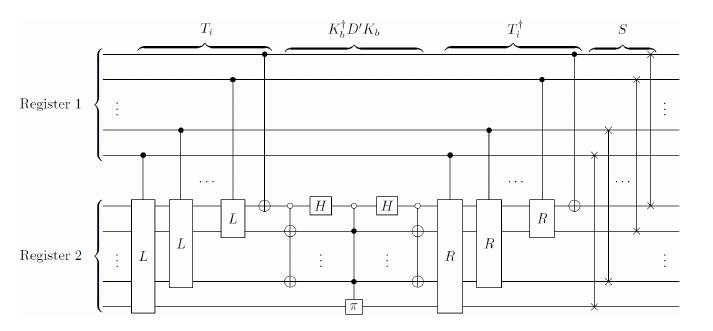
\includegraphics[scale=0.5]{img/generic_szegedy.jpg}
        \centering
    \end{figure}
\end{frame}

\begin{frame}
    \frametitle{Circuit for the specific Szegedy QW on a cycle graph}
    \begin{figure}[h!]
        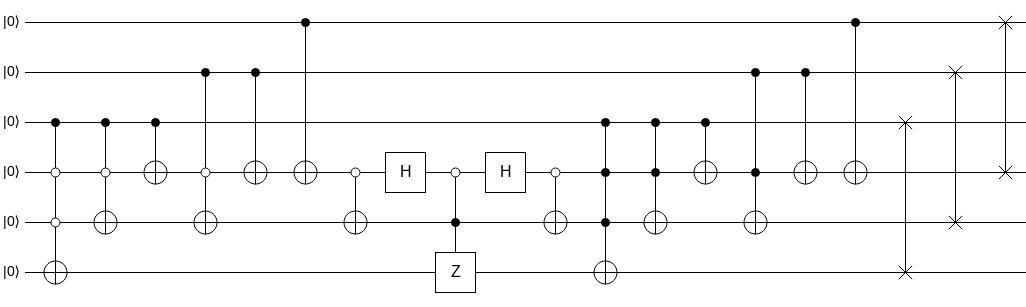
\includegraphics[scale=0.4]{img/szegedy_c8.jpg}
        \centering
    \end{figure}
    \href{https://bit.ly/2X3PvAk}{Here the Quirk Simulation}
\end{frame}

\begin{frame}
    \frametitle{Applications}
    Methods presented can be used and adapted to different areas, some 
    example that i found are:
    \begin{itemize}
        \item NP hard solved with randomized algorithms
        \item Quantum page rank
        \item Hybrid linear system solver
    \end{itemize}
\end{frame}

\begin{frame}
    \frametitle{The End}

    Thank you for your attention!

\end{frame}

\end{document}